\documentclass[journal,twoside,web]{ieeecolor}
\usepackage{generic}
\usepackage{cite}
\usepackage{amsmath,amssymb,amsfonts}
\usepackage{algorithm}
\usepackage{algorithmic}
\usepackage{graphicx}
\usepackage{textcomp}
\usepackage{booktabs}
\usepackage{tabularx}
\usepackage{multirow}
\graphicspath{{figures/}}
\def\BibTeX{{\rm B\kern-.05em{\sc i\kern-.025em b}\kern-.08em
    T\kern-.1667em\lower.7ex\hbox{E}\kern-.125emX}}
\markboth{\journalname, VOL. XX, NO. XX, XXXX}
{Author \MakeLowercase{\textit{et al.}}: Title}
\begin{document}
\title{A Dual-Graph Counterfactual MAPPO Framework for Dynamic Multi-Robot Navigation}
\author{First A. Author, \IEEEmembership{Fellow, IEEE}, Second B. Author, and Third C. Author, Jr., \IEEEmembership{Member, IEEE}
\thanks{}
\thanks{}
\thanks{}
\thanks{}}

\maketitle

\begin{abstract}
Multi-agent reinforcement learning (MARL) provides a principled means of coordinating autonomous ground vehicles (AGVs) in shared warehouse and logistics environments. Two obstacles, however, limit its effectiveness in dense traffic. Shared team rewards supply only weak individual credit when agent interactions are tightly coupled, and the deep integration of graph operators into the policy network introduces non-stationarity that destabilizes optimization. This article proposes a dual-graph counterfactual variant of multi-agent proximal policy optimization (MAPPO) that addresses both obstacles. A rolling-subgoal planner with adaptive detour logic decouples long-horizon routing from local conflict resolution. Two ego-centric graphs, one for social risk among neighboring agents and one for dynamic obstacle motion, each attend to a small set of high-risk entities. Neighboring agents are selected by proximity, dynamic obstacles by a composite risk score that incorporates predicted time-to-collision, and both graphs are processed by a risk-biased graph attention network. A residual gate blends the resulting graph features into a stable multilayer-perceptron and long short-term memory (MLP--LSTM) navigation backbone only when interaction risk is elevated, which preserves training stability in open spaces. A leave-one-out counterfactual critic estimates the marginal contribution of each agent to the team value and injects this contribution into the per-agent reward before advantage estimation, thereby sharpening cooperative credit without dual value heads or explicit value factorization. A partial-done training protocol with density-adaptive reward scaling maintains consistent trajectory semantics across team sizes ranging from two to eight robots. In Gazebo Circle-Swap evaluations, the framework improves the success rate and the minimum inter-agent separation relative to a backbone-only baseline, a fully connected graph baseline, and the classical optimal reciprocal collision avoidance (ORCA) baseline. Ablation studies confirm that each component contributes measurably to the final performance.
\end{abstract}

\begin{IEEEkeywords}
Multi-robot navigation, multi-agent reinforcement learning, graph attention networks, counterfactual credit assignment, curriculum learning.
\end{IEEEkeywords}

\section{Introduction}
\label{sec:introduction}
\IEEEPARstart{I}{n} modern warehouse automation, logistics centers, and factory floors, autonomous ground vehicles (AGVs) operate in shared spaces to transport materials and sustain production throughput. Each vehicle must navigate from its current position to a dynamically assigned goal while avoiding static infrastructure, moving obstacles such as forklifts and human workers, and other vehicles pursuing their own goals. The difficulty is not merely geometric obstacle avoidance; it lies in resolving strongly coupled interactions such as head-on encounters in narrow aisles, merging conflicts at intersections, and congestion in high-traffic zones under partial observability. As fleet density grows to meet throughput demands, small improvements in collision avoidance and coordination translate directly into operational uptime and safety margins.

Classical reactive methods such as reciprocal velocity obstacles (RVO) and optimal reciprocal collision avoidance (ORCA)~\cite{vandenberg2008rvo,vandenberg2011orca} are computationally efficient and interpretable, but they optimize only instantaneous local feasibility and cannot exploit interaction history. Deep reinforcement learning (DRL) jointly optimizes perception, local control, and multi-step interaction reasoning, with decentralized learners~\cite{chen2017decentralized,long2018towards,fan2020distributed}, light detection and ranging (LiDAR) based perception~\cite{liu2024saclidar,zhang2025complicated}, memory-augmented architectures~\cite{montero2025memory}, and path-constrained planning~\cite{pico2025pathconstrained,meng2025robust} all advancing the state of the art~\cite{chen2025survey}. Graph neural networks (GNNs) and attention mechanisms have been introduced to capture pairwise dependencies among agents~\cite{zhang2025gatmapf,escudie2024multisoc,bi2025decentralized,liu2025cooperative,xiao2024macns,wong2024mrnppo,wang2025parallelcooperative}. Two challenges nevertheless persist. First, deep graph integration couples the evolving policy and the graph feature space, injecting non-stationarity that disrupts the trust-region updates of proximal policy optimization (PPO). Second, shared team rewards provide weak individual credit signals, so the centralized critic of multi-agent PPO (MAPPO) struggles to discriminate which agent's action caused a success or failure in tightly coupled events.

We address both issues with a dual-graph counterfactual MAPPO framework that separates stable local navigation from selective relational reasoning. Two lightweight ego-centric graphs, one for social risk and one for dynamic obstacles, each attend only to a small set of high-risk entities: neighboring agents are selected by proximity, whereas dynamic obstacles are selected by a composite risk score that incorporates predicted time-to-collision (TTC). A residual fusion gate modulates a multilayer-perceptron and long short-term memory (MLP--LSTM) backbone only when conflict risk is elevated. A leave-one-out counterfactual critic estimates the marginal contribution of each agent to the team value and injects this contribution into the per-agent reward before generalized advantage estimation (GAE), which requires one additional forward pass per agent and no dual value heads. A rolling-subgoal planner with adaptive detour logic offloads path following, and a partial-done protocol with density-adaptive reward scaling sustains consistent trajectory semantics from two to eight robots. The contributions of this article are as follows.
\begin{enumerate}
    \item \textbf{Dual-graph attention for decoupled risk reasoning.} We separate social interaction and dynamic obstacle avoidance into two ego-centric attention graphs, each attending to high-risk entities selected by proximity or by predictive motion descriptors. This architectural decoupling permits clean component-level ablation and prevents cross-contamination between the learning signals for neighbor coordination and obstacle avoidance.
    \item \textbf{Residual fusion with risk-aware gating.} Unlike prior graph-based navigation methods that route all observations through graph layers~\cite{zhang2025gatmapf,escudie2024multisoc}, we retain the MLP--LSTM backbone and use a learned sigmoid gate that admits graph features only when social or obstacle risk is elevated. This design maintains training stability in low-conflict regions while enabling graph reasoning where it is required.
    \item \textbf{Leave-one-out counterfactual credit.} We inject single-permutation Monte Carlo Shapley estimates into the per-agent reward before advantage estimation, which sharpens cooperative learning under shared rewards without dual critics or explicit value factorization.
    \item \textbf{Density-adaptive training protocol.} We pair a partial-done scheme with reward scaling that varies as the square root of the team size, which yields consistent learning signals across scenarios ranging from two to eight robots and addresses the scalability limitation of fixed-reward MARL formulations.
\end{enumerate}

\section{Related Work}
\label{sec:related_work}

\textbf{MARL for navigation.} Decentralized learners~\cite{chen2017decentralized,long2018towards} demonstrated self-play collision avoidance but suffer from non-stationarity as each agent's policy evolves. Value-decomposition methods such as QMIX~\cite{rashid2018qmix} and QTRAN factorize the joint action-value function under monotonicity constraints, but they are confined to discrete actions and require careful architectural design. MAPPO~\cite{yu2022mappo} combines a shared policy with a centralized critic for training under the centralized-training-with-decentralized-execution (CTDE) paradigm and has been applied to continuous-control navigation~\cite{fan2020distributed}; however, its shared reward provides only indirect individual credit, which is especially acute in head-on encounters where yielding and proceeding receive identical signals. The counterfactual multi-agent policy gradient (COMA)~\cite{foerster2018coma} computes counterfactual baselines but needs one critic pass per discrete action per agent, making it prohibitive for continuous control. We instead estimate per-agent marginal contributions by masking the agent's observation slot inside the centralized critic, and we inject those contributions into the reward channel before advantage estimation. This requires only one extra critic pass per agent while preserving gradient flow under importance sampling.

\textbf{Graph reasoning in multi-robot systems.} CommNet~\cite{sukhbaatar2016commnet} and TarMAC~\cite{das2019tarmac} use message-passing architectures with fixed or learned weights but lack explicit risk modeling. The graph attention network (GAT)~\cite{velickovic2018gat} introduces data-dependent attention and has been applied to multi-robot planning~\cite{zhang2025gatmapf} and cooperative navigation~\cite{escudie2024multisoc,bi2025decentralized}. Hierarchical~\cite{liu2025cooperative}, centralized~\cite{xiao2024macns}, and parallel-cooperative~\cite{wong2024mrnppo} graphs further demonstrate the value of relational structure, but they typically embed graph operators deep inside the policy and conflate neighbor coordination with obstacle avoidance into a single graph. Our dual-graph design separates these two reasoning patterns and lets graph features modulate—rather than replace—the navigation backbone via a residual gate, recognizing that social coordination is reciprocal and game-theoretic while obstacle avoidance is a unilateral prediction problem.

\textbf{Credit assignment and density adaptation.} Difference rewards~\cite{wolpert2002optimal} estimate per-agent contributions but require expensive counterfactual rollouts. Exact Shapley values~\cite{shapley1953value} are exponential in the number of agents, motivating sampling-based approximations~\cite{wang2020shapley} and structural decompositions~\cite{chang2022shapley} that nevertheless require separate value networks. We use a single-permutation Monte Carlo Shapley estimator that adds no parameters: the centralized critic is queried twice per agent, once on the full global state and once with that agent's observation masked. Safety-critical~\cite{zhu2025safehj,dawood2025safecoop} and robust planning~\cite{riemens2026gpmpc} frameworks address worst-case guarantees but do not explicitly model how credit and reward weights should scale with team size; we close this gap with a square-root density factor that scales collision penalties and social weights to keep learning signals consistent across team sizes.

\section{Problem Statement}
\label{sec:problem_statement}

We consider $N$ homogeneous mobile robots operating in a two-dimensional workspace $\mathcal{W}\subset\mathbb{R}^2$ shared with static obstacles, other robots, and dynamic obstacles. Each robot $i$ has state $s_t^i=[p_t^i,v_t^i,\theta_t^i,\omega_t^i]$, where $p_t^i\in\mathbb{R}^2$ is the planar position, $v_t^i$ the linear velocity, $\theta_t^i$ the heading, and $\omega_t^i$ the angular velocity; the global state is $s_t=(s_t^1,\ldots,s_t^N)$. Each robot executes continuous actions $a_t^i=[u_{v,t}^i,u_{\omega,t}^i]$ commanding linear and angular velocities and receives a local observation $o_t^i$ that aggregates its sensor readings, the current rolling subgoal, and received neighbor information; the exact composition of $o_t^i$ is given in Section~\ref{sec:obs}.

The task is modeled as a decentralized partially observable Markov decision process (Dec-POMDP) $\mathcal{M}=\bigl\langle\mathcal{A},\mathcal{S},\{\mathcal{O}^i\},\{\mathcal{U}^i\},\mathcal{P},\mathcal{R},\gamma\bigr\rangle$~\cite{oliehoek2016concise,bernstein2002complexity} and trained under the CTDE paradigm. A shared decentralized policy $\pi_\theta(a_t^i\mid o_t^i,h_t^i)$ with recurrent state $h_t^i$ is executed locally, while a centralized critic $V_\psi(s_t)$ is used only during training to supply global value estimates. The optimization objective is the discounted expected return $J(\theta)=\mathbb{E}_{\pi_\theta}\!\bigl[\sum_{t=0}^{T}\gamma^t r_t\bigr]$ under a shared team reward $r_t=\sum_i r_t^i$.

\section{Method}
\label{sec:method}

\begin{figure}[t]
\centering
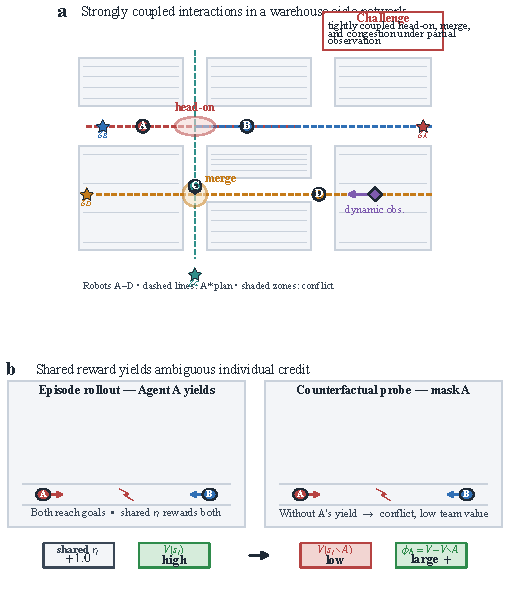
\includegraphics[width=\columnwidth]{figures/fig2_motivation_scenario.pdf}
\caption{\textbf{Motivation.} (a)~Warehouse aisle network in which multiple AGVs face tightly coupled head-on, merging, and dynamic-obstacle conflicts under partial observability. (b)~Under a shared team reward $r_t$, both agents that participate in a head-on encounter receive identical credit even though only one yielded; the counterfactual signal $\phi_A = V(s_t) - V(s_t\setminus A)$ resolves this ambiguity by quantifying each agent's marginal contribution to team value.}
\label{fig:motivation}
\end{figure}

\begin{figure*}[t]
\centering
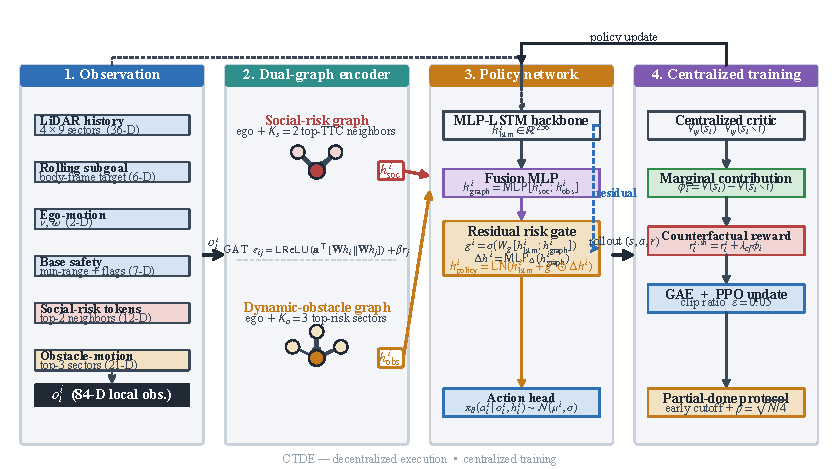
\includegraphics[width=\textwidth]{figures/fig1_system_architecture.pdf}
\caption{\textbf{System architecture of the dual-graph counterfactual MAPPO framework.} The pipeline consists of four stages. (1)~\emph{Observation construction} extracts rolling subgoals from a global A* planner and combines them with a local occupancy map, ego-motion, and neighbor information to form the local observation. (2)~\emph{Dual-graph encoding} constructs two ego-centric graphs, namely a social-risk graph that attends to the nearest neighbors and a dynamic-obstacle graph that attends to moving obstacles via motion descriptors, and processes them with separate GAT encoders. (3)~\emph{Policy network} fuses the MLP--LSTM navigation backbone with the dual-graph features through a residual gate, producing continuous velocity commands. (4)~\emph{Centralized training} uses a leave-one-out counterfactual critic to estimate the marginal contributions $\phi_i = V(s) - V(s \setminus i)$, which are injected into the per-agent rewards before advantage estimation. The partial-done protocol terminates an episode early when the number of active agents drops below a threshold, which maintains clean trajectory boundaries for PPO updates.}
\label{fig:system_architecture}
\end{figure*}

Building on the Dec-POMDP formulation of Section~\ref{sec:problem_statement}, we train decentralized policies $\pi_\theta(a_t^i\mid o_t^i,h_t^i)$ with a centralized critic $V_\psi(s_t)$ under PPO. The framework integrates four components: rolling-subgoal guidance (Section~\ref{sec:rolling}), dual-graph attention (Section~\ref{sec:dual_graph}), residual risk-gated fusion (Section~\ref{sec:policy_arch}), and leave-one-out counterfactual credit assignment (Section~\ref{sec:counterfactual}). Figure~\ref{fig:system_architecture} illustrates the pipeline.

\subsection{Rolling-Subgoal Guidance with Adaptive Detour Logic}
\label{sec:rolling}

An end-to-end policy must simultaneously infer long-horizon path progression and resolve local conflicts. This dual burden slows learning and induces myopic oscillation near obstacles. We therefore decouple path-level guidance from interaction-level control: a deterministic A* planner provides geometric routing, while the learned policy specializes in conflict resolution. At each timestep, agent $i$ projects its current position onto the precomputed path and selects a look-ahead point $g_t^i$ at an adaptive distance
\[
L_{\text{adapt}} = L_0 \, f_{\text{front}}(d_{\min}) \, g_{\text{heading}}(\Delta\theta),
\]
where $L_0 = 0.8$\,m is the nominal look-ahead, $f_{\text{front}}$ reduces $L_{\text{adapt}}$ when the front LiDAR sector reports a minimum range below $0.5$\,m, and $g_{\text{heading}}$ reduces it when the heading error exceeds $30^\circ$. The subgoal is expressed in the body frame of the robot as a three-element descriptor that encodes the clipped distance and the sine and cosine of the bearing.

When the corridor ahead is blocked, which is defined as a front range below $0.42$\,m together with side clearances below $0.20$\,m, a detour rule overrides the nominal subgoal with the widest gap within $\pm 60^\circ$ and holds it for eight timesteps to suppress oscillation. The rolling subgoal therefore provides a stable heading and progress reference for the policy and offloads path following from the recurrent backbone.

%------------------------------------------------------------------------------
\subsection{Observation Construction and Risk-Based Token Selection}
\label{sec:obs}

The local observation $o_t^i$ comprises a base feature vector and a local occupancy map. The base feature vector concatenates five groups. The \emph{rolling-subgoal block} contains the body-frame target descriptor of Section~\ref{sec:rolling} together with the goal distance, the goal bearing, and the path-progress ratio (six dimensions). \emph{Ego-motion} adds the linear and angular velocities (two dimensions). The \emph{base safety block} encodes the global minimum range and the front minimum range (two dimensions). The \emph{social-risk tokens} retain up to two neighboring agents, and the \emph{obstacle-motion tokens} retain up to three dynamic obstacles, as detailed below. An \emph{agent-identity block} appends a one-hot agent index (eight dimensions) to break symmetry among homogeneous robots. These groups yield a base feature vector of $6+2+2+14+21+8=53$ dimensions. In parallel, a local occupancy map of two stacked frames over a $32\times32$ grid (2048 dimensions) is encoded by a small convolutional network and provides the spatial context that replaces an explicit raw-scan history.

The \emph{social-risk tokens} are populated by proximity-based selection. Among the neighbors within the communication range, the two nearest are retained; each token is seven-dimensional and encodes the body-frame relative position, the body-frame relative velocity, the normalized distance, and the sine and cosine of the relative heading, giving fourteen dimensions in total. The \emph{obstacle-motion tokens} are populated by risk-based selection. For each detected dynamic obstacle, a composite risk score is computed from the current distance, the predicted future distance, a crossing-risk term, and a predicted time-to-collision term; the three highest-risk obstacles are retained. Each token is seven-dimensional and encodes the current body-frame position, the body-frame velocity, the predicted future position, and a binary dynamic flag, giving twenty-one dimensions in total. This selection ensures that the graph attention layers introduced next concentrate their computational budget on entities that pose immediate collision risk rather than on all visible neighbors. All features are normalized to $[-1,1]$ or $[0,1]$. The centralized critic concatenates the base feature vectors of all agents to construct the global state.

%------------------------------------------------------------------------------
\subsection{Dual-Graph Attention Architecture}
\label{sec:dual_graph}

\begin{figure}[t]
\centering
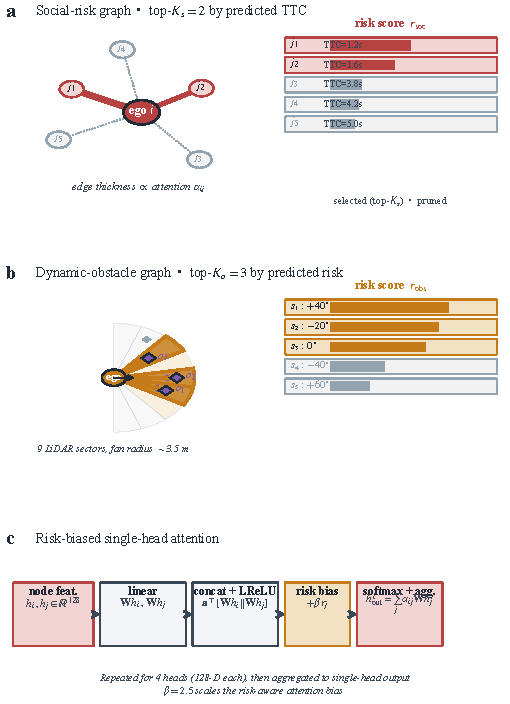
\includegraphics[width=\columnwidth]{figures/fig3_dual_graph_attention.pdf}
\caption{\textbf{Dual-graph attention.} (a)~Social-risk graph: the ego attends to the top-$K_s{=}2$ nearest neighbors; pruned candidates are shown dashed and edge thickness encodes the resulting attention weight $\alpha_{ij}$. (b)~Dynamic-obstacle graph: the ego attends to the top-$K_o{=}3$ dynamic obstacles, each scored by proximity, predicted future distance, and closing rate. (c)~One head of the risk-biased GAT: features are linearly projected, concatenated with a leaky-rectified compatibility score, augmented by a per-neighbor risk bias $\beta\, r_j$ with $\beta{=}2.5$, and softmax-normalized to yield $\alpha_{ij}$ before the value features are aggregated.}
\label{fig:dual_graph}
\end{figure}

Treating all pairwise interactions uniformly conflates two distinct reasoning tasks. Coordinating with neighboring agents is reciprocal and benefits from game-theoretic modeling, whereas avoiding dynamic obstacles is essentially a unilateral prediction problem. Mixing the two into a single graph forces the network to learn entangled representations and weakens credit assignment under ablation. We therefore construct two ego-centric graphs and process them with independent GAT encoders.

The \emph{social-risk graph} $\mathcal{G}_{\text{social}}^i$ contains the ego node together with up to $K_s = 2$ nearest neighbors selected from the social-risk tokens. The ego features are obtained from the base observation by a two-layer perceptron, each neighbor's seven-dimensional social-risk token is encoded by a shared two-layer perceptron, and both branches are projected to a 128-dimensional embedding. Edges connect the ego to each valid neighbor, and the attention logits are biased by a proximity-derived risk score,
\[
e_{ij} = \mathrm{LeakyReLU}\!\bigl(\mathbf{a}^\top[\mathbf{W}h_i\,\Vert\,\mathbf{W}h_j]\bigr) + \beta\, r_{\text{social}}^{\,j},
\]
where the risk-bias coefficient is $\beta = 2.5$ and $r_{\text{social}}^{\,j}$ increases as the neighbor approaches. The bias ensures that high-risk neighbors receive larger attention weights even when their features are not the most similar to those of the ego. A four-head GAT layer with 128-dimensional per-head representations, followed by single-head aggregation, produces the social embedding $h_{\text{social}}^i\in\mathbb{R}^{128}$.

The \emph{dynamic-obstacle graph} $\mathcal{G}_{\text{obstacle}}^i$ shares the same ego encoding and uses an analogous attention bias $\beta\, r_{\text{obstacle}}^{\,j}$ over up to $K_o = 3$ obstacle tokens, where $r_{\text{obstacle}}^{\,j}$ combines proximity, predicted future distance, and a crossing-risk term. Each token is seven-dimensional and is encoded to a 128-dimensional vector by a separate shared perceptron. The obstacle GAT has independent parameters and produces the obstacle embedding $h_{\text{obstacle}}^i\in\mathbb{R}^{128}$.

The architecture supports three configurations used in our ablations: a \emph{social-only} variant that uses $h_{\text{social}}^i$ alone, an \emph{obstacle-only} variant that uses $h_{\text{obstacle}}^i$ alone, and the \emph{dual-graph} variant that fuses both embeddings as described in Section~\ref{sec:policy_arch}. This separation allows each graph's contribution to be isolated cleanly during experimental evaluation.

%------------------------------------------------------------------------------
\subsection{Policy Network with Residual Risk-Gated Fusion}
\label{sec:policy_arch}

\begin{figure}[t]
\centering
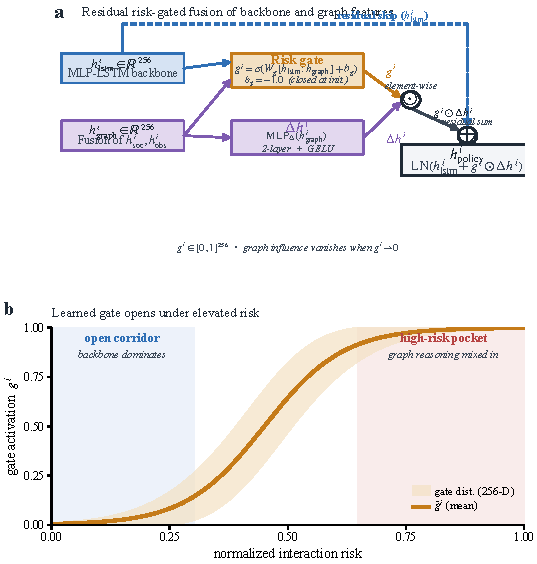
\includegraphics[width=\columnwidth]{figures/fig4_residual_gate.pdf}
\caption{\textbf{Residual risk-gated fusion.} (a)~The MLP--LSTM backbone embedding $h^i_{\mathrm{lstm}}$ bypasses the graph encoder via a residual skip. The fused graph embedding $h^i_{\mathrm{graph}}$ is transformed by $\mathrm{MLP}_\Delta$ and modulated element-wise by a learned sigmoid gate $g^i = \sigma(W_g[h^i_{\mathrm{lstm}};h^i_{\mathrm{graph}}]+b_g)$, with the bias $b_g = -1.0$ keeping the gate near zero at initialization. The gated delta is added to $h^i_{\mathrm{lstm}}$ and normalized to yield $h^i_{\mathrm{policy}}$. (b)~Mean gate activation $\bar g^i$ as a function of normalized interaction risk: in open corridors (left band) the backbone dominates, while in high-risk pockets (right band) graph reasoning is mixed in.}
\label{fig:residual_gate}
\end{figure}

Directly replacing the MLP backbone with a graph encoder introduces non-stationarity during training: as the policy evolves, neighbor behaviors change, the graph feature distribution shifts, and the trust-region updates of PPO become unstable. Earlier work addresses this issue by freezing the graph parameters or by training in separate phases, but both approaches sacrifice adaptability. We instead retain a stable MLP--LSTM backbone for routine navigation and allow the graph features to modulate the output only when interaction risk is elevated.

The policy processes observations in three stages. In the first stage, the base features, the convolutional embedding of the local occupancy map, and the neighbor features are concatenated, normalized, and fed into a long short-term memory cell with hidden dimension 256,
\[
h_t^i,\, c_t^i = \mathrm{LSTM}(o_t^i,\, h_{t-1}^i,\, c_{t-1}^i).
\]
A reset flag gates the recurrent state: when an agent respawns after reaching a goal or colliding, its hidden state is zeroed to prevent contamination across trajectory segments. The output is then normalized to produce a stable temporal feature $h_{\text{lstm}}^i\in\mathbb{R}^{256}$.

In the second stage, the social and obstacle graph embeddings are projected to 256 dimensions through separate linear layers with Gaussian-error-linear-unit activations. In the dual-graph configuration the two embeddings are concatenated and fused by a two-layer perceptron into $h_{\text{graph}}^i\in\mathbb{R}^{256}$; the social-only and obstacle-only configurations reuse the corresponding embedding directly.

In the third stage, a learned sigmoid gate determines how much graph influence to blend into the backbone,
\[
\begin{aligned}
g^i &= \sigma\!\bigl(\mathbf{W}_g[h_{\text{lstm}}^i;\,h_{\text{graph}}^i]+\mathbf{b}_g\bigr),\\
\Delta h^i &= \mathrm{MLP}_\Delta(h_{\text{graph}}^i),\\
h_{\text{policy}}^i &= \mathrm{LayerNorm}\!\bigl(h_{\text{lstm}}^i + g^i\odot\Delta h^i\bigr),
\end{aligned}
\]
where $g^i\in[0,1]^{256}$ is element-wise and $\odot$ denotes the Hadamard product. The gate bias $\mathbf{b}_g$ is initialized to $-1.0$ so that the gate starts near zero; the policy therefore begins as an MLP--LSTM and learns to open the gate where graph reasoning is useful. The fused feature drives a linear head that produces the mean $\boldsymbol{\mu}^i$ of a diagonal Gaussian action distribution. The log-standard-deviation is produced by the same head and clamped to $[-5.0, 0.5]$ to prevent entropy collapse or explosion in late training.

%------------------------------------------------------------------------------
\subsection{Leave-One-Out Counterfactual Credit Assignment}
\label{sec:counterfactual}

\begin{figure}[t]
\centering
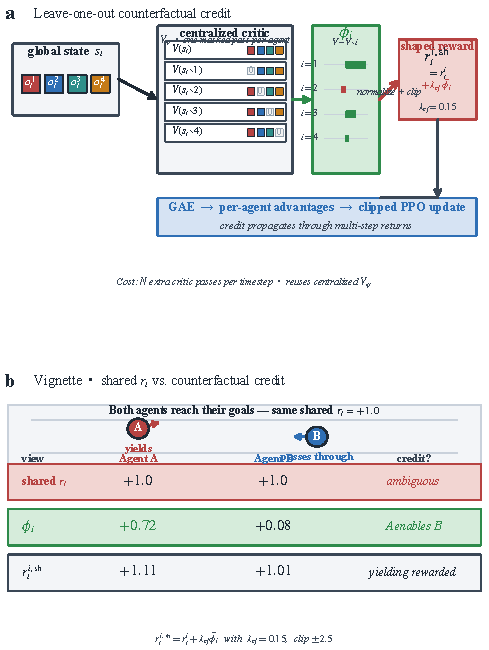
\includegraphics[width=\columnwidth]{figures/fig5_counterfactual_credit.pdf}
\caption{\textbf{Leave-one-out counterfactual credit.} (a)~At each timestep the centralized critic computes the value of the full global state $V(s_t)$ and $N$ masked variants $V(s_t\setminus i)$ in which agent $i$'s observation slot is zeroed; the marginal contributions $\phi_i = V(s_t) - V(s_t\setminus i)$ are normalized, clipped, scaled by $\lambda_{cf}{=}0.15$, and injected into per-agent rewards before advantage estimation so that the credit propagates through multi-step returns. (b)~Vignette of a head-on encounter: under a shared $r_t$ both agents look identical, while $\phi_i$ assigns the larger positive credit to the yielding agent, breaking the credit ambiguity.}
\label{fig:counterfactual}
\end{figure}

Standard MAPPO uses a shared team reward $r_t=\sum_i r_t^i$ and a centralized critic $V(s_t)$, so individual agents receive identical reward signals. In tightly coupled events such as head-on encounters, the agent that yields and the agent that proceeds receive the same credit. Value factorization methods such as QMIX~\cite{rashid2018qmix} and counterfactual baselines such as COMA~\cite{foerster2018coma} address this through per-agent baselines or factorized critics, at the cost of additional architecture.

We instead implement a single-permutation Monte Carlo Shapley estimator and inject the marginal contribution into the reward channel rather than the advantage. For each agent $i$, the centralized critic computes two values: the value of the full state $V(s_t)$, and a counterfactual value $V(s_t\setminus i)$ in which the slot of agent $i$ within the global state is zeroed by a binary node mask. The marginal contribution is
\[
\phi_i(s_t) = V(s_t) - V(s_t\setminus i),
\]
and the shaped per-agent reward is
\[
r_t^{i,\text{sh}} = r_t^i + \lambda_{\text{cf}}\,\mathrm{clip}\!\Bigl(\tfrac{\phi_i(s_t)-\mu_\phi}{\sigma_\phi+\epsilon},\,-c,\,c\Bigr),
\]
where $\lambda_{\text{cf}}=0.15$ is the credit coefficient, $(\mu_\phi,\sigma_\phi)$ are the batch statistics used for normalization, $c=2.5$ is the clip threshold, and $\epsilon=10^{-6}$ avoids division by zero. Standard generalized advantage estimation then propagates the credit through multi-step returns. Injecting $\phi_i$ into the reward before advantage estimation, rather than adding it directly to the advantage where it would have no gradient effect under importance sampling, preserves clean policy-gradient semantics, requires only one additional critic pass per agent, and reuses the existing centralized critic without introducing dual value heads.

%------------------------------------------------------------------------------
\subsection{Density-Adaptive Reward and Partial-Done Training Protocol}
\label{sec:training_protocol}

As the team size grows from two to eight robots, the collision probability and the congestion severity rise nonlinearly with density, so a fixed reward weight either under-penalizes collisions in dense regimes or over-penalizes them in sparse ones. In addition, standard episode termination, which waits for all agents to finish, prolongs episodes when some agents have completed their goals while others remain stuck, which dilutes the training signal.

We scale the collision penalty and the social reward weight by a density factor $\rho=\sqrt{N/4}$ with a baseline team size of four,
\[
r_{\text{collision}} = -20.0\bigl(1+0.2(\rho-1)\bigr),\qquad w_{\text{social}} = 1.0\,\rho.
\]
The square-root scaling keeps the gradient informative without over-penalizing dense settings: for $N=8$, $\rho\approx 1.41$ yields a collision penalty of $-28.2$ and a social weight of $1.41$. An agent transitions to the done state upon reaching its goal or colliding, and the episode terminates early once the number of still-active agents drops below $N_{\min}=2$ or the number of failed agents exceeds $N_{\text{fail}}=2$. Combined with the per-agent recurrent-state resets of Section~\ref{sec:policy_arch}, this protocol produces clean PPO trajectory boundaries and prevents degenerate post-failure states from dominating the rollout buffer.

Algorithm~\ref{alg:training} summarizes one full iteration of the training loop. The actor branch is unchanged from standard MAPPO; the only additions are the dual-graph forward pass, the leave-one-out critic pass, and the reward-shaping step that is applied before advantage estimation. The cost of the additional critic passes is linear in the number of agents but reuses the same network weights, so the memory footprint is unchanged.

\begin{algorithm}[t]
\caption{Dual-graph counterfactual MAPPO (one iteration).}
\label{alg:training}
\begin{algorithmic}[1]
\REQUIRE policy $\pi_\theta$, centralized critic $V_\psi$, batch of $M$ trajectories
\FORALL{$(o_t^i,s_t,a_t,r_t,\mathrm{reset}_t)$ in the batch}
  \STATE encode $h_{\text{lstm}}^i\!\gets\!\mathrm{LSTM}(o_t^i,h_{t-1}^i)$ with reset gating
  \STATE build risk tokens; run the dual GAT to obtain $h_{\text{social}}^i,h_{\text{obstacle}}^i$
  \STATE fuse, gate, and output $\boldsymbol{\mu}^i$ as in Section~\ref{sec:policy_arch}
  \STATE evaluate $V(s_t)\!\gets\!V_\psi(s_t)$ and $V(s_t\!\setminus\!i)\!\gets\!V_\psi(\mathrm{mask}_i(s_t))$
  \STATE $\phi_i(s_t)\gets V(s_t)-V(s_t\!\setminus\!i)$
\ENDFOR
\STATE normalize and clip $\widetilde\phi_i$; shape $r_t^{i,\text{sh}}\!\gets\!r_t^i+\lambda_{\text{cf}}\widetilde\phi_i$
\STATE compute GAE advantages from $\{r_t^{i,\text{sh}}\}$, bootstrap with $V(s_t)$
\STATE update $\theta$ with the clipped PPO objective; update $\psi$ on returns
\STATE apply the partial-done cutoff if $N_{\text{active}}<N_{\min}$ or $N_{\text{fail}}>N_{\text{fail}}^\star$
\end{algorithmic}
\end{algorithm}

%------------------------------------------------------------------------------

\section{Experimental Setup}
\label{sec:experiments}

\subsection{Simulator and Training Configuration}
\label{sec:setup_train}

Experiments are conducted in the Gazebo simulator under Robot Operating System 2 (ROS 2) Humble, using TurtleBot3 Burger platforms (wheelbase $0.16$\,m, maximum linear velocity $0.22$\,m/s, maximum angular velocity $2.84$\,rad/s). The LDS-01 LiDAR provides $360^\circ$ scans at $5$\,Hz with a $3.5$\,m range; these scans are rasterized into the local occupancy map of Section~\ref{sec:obs} that the policy consumes. Training is performed with Ray RLlib~2.5 using PPO. The principal hyperparameters and architecture sizes are summarized in Table~\ref{tab:hyperparams}. Every configuration is evaluated over one hundred test episodes with three independent random seeds.

\begin{table}[t]
\centering
\caption{Hyperparameters and architecture sizes.}
\label{tab:hyperparams}
\renewcommand{\arraystretch}{1.05}
\setlength{\tabcolsep}{6pt}
\begin{tabularx}{\columnwidth}{l X r}
\toprule
Group & Parameter & Value \\
\midrule
\multirow{5}{*}{PPO}
 & Learning rate                    & $3\times10^{-5}$ \\
 & Clip $\epsilon$                  & $0.05$ \\
 & GAE $\lambda$, discount $\gamma$ & $0.95$, $0.99$ \\
 & Entropy coefficient              & $0.005$ \\
 & Batch / rollout                  & $5000$ / $1000$ \\
\midrule
\multirow{4}{*}{Network}
 & LSTM hidden size                 & $256$ \\
 & GAT heads / dim                  & $4$ / $128$ \\
 & Top-$K_s$ / top-$K_o$            & $2$ / $3$ \\
 & Action $\log\sigma$ clamp        & $[-5.0,\,0.5]$ \\
\midrule
\multirow{3}{*}{Credit \& gate}
 & $\lambda_{\text{cf}}$            & $0.15$ \\
 & Clip $c$ for $\widetilde\phi_i$  & $2.5$ \\
 & Gate bias $b_g$                  & $-1.0$ \\
\midrule
\multirow{3}{*}{Training}
 & Density factor                   & $\rho=\sqrt{N/4}$ \\
 & $N_{\min},\,N_{\text{fail}}$     & $2$, $2$ \\
 & Workers / seeds                  & $8$ / $3$ \\
\bottomrule
\end{tabularx}
\end{table}

\subsection{Scenarios and Curriculum}
\label{sec:setup_scenarios}

We evaluate on three Circle-Swap scenarios of increasing density. Circle-Swap-$2$ places two robots that swap positions diagonally across an $8\,\text{m}\times 8\,\text{m}$ arena with three dynamic obstacles moving at $0.15$\,m/s, and tests basic collision avoidance and symmetry breaking. Circle-Swap-$4$ places four robots in antipodal pairs with four dynamic obstacles at $0.18$\,m/s, introducing multi-body interactions and coordinated yielding. Circle-Swap-$8$ has eight robots in high-density swapping with five dynamic obstacles at $0.21$\,m/s and stresses both the credit assignment mechanism and the density-adaptive reward. Training follows a six-stage curriculum that progressively increases team size and obstacle count, summarized in Table~\ref{tab:curriculum}. Each stage is trained until the moving-average return plateaus, and the next stage is initialized from the previous stage's checkpoint.

\begin{table}[t]
\centering
\caption{Six-stage curriculum schedule used during training.}
\label{tab:curriculum}
\renewcommand{\arraystretch}{1.05}
\setlength{\tabcolsep}{4pt}
\begin{tabularx}{\columnwidth}{c c c c c X}
\toprule
Stage & $N$ & Dynamic obs. & Arena (m) & Steps (k) & Focus \\
\midrule
$1$ & $2$ & $0$ & $6\!\times\!6$  & $200$ & Basic navigation \\
$2$ & $2$ & $2$ & $8\!\times\!8$  & $250$ & Obstacle avoidance \\
$3$ & $4$ & $3$ & $8\!\times\!8$  & $350$ & Coordination \\
$4$ & $4$ & $4$ & $8\!\times\!8$  & $450$ & Head-on resolution \\
$5$ & $6$ & $4$ & $10\!\times\!10$ & $500$ & Multi-body congestion \\
$6$ & $8$ & $5$ & $10\!\times\!10$ & $600$ & Dense flow \\
\bottomrule
\end{tabularx}
\end{table}

\subsection{Baselines, Ablations, and Metrics}
\label{sec:setup_baselines}

We compare against three baselines. The \emph{MLP--LSTM backbone} keeps only the navigation backbone with the residual gate held closed, isolating the contribution of all graph and counterfactual components. The \emph{fully connected graph baseline} replaces our dual-graph encoder with a single GAT operating over every neighbor within $3.5$\,m, representing the prevailing communication-graph design in prior multi-robot work. The \emph{ORCA baseline} couples the classical optimal reciprocal collision avoidance controller with A* path following and represents the rule-based state of the art.

Four ablations isolate the role of each component of the proposed framework. The \emph{no-counterfactual} variant disables the counterfactual reward by setting $\lambda_{\text{cf}}=0$ while retaining the dual-graph encoder. The \emph{social-only} and \emph{obstacle-only} variants restrict the architecture to a single graph branch. The \emph{no-gate} variant replaces the residual risk gate with direct concatenation of the backbone and graph embeddings.

We report four metrics. Success rate (SR) is the percentage of agents that reach their goals within the episode time limit. Collision rate (CR) is the percentage of agents that collide with obstacles or other agents. Episode length (EL) is the mean number of timesteps to completion, where smaller values indicate more efficient navigation. Minimum inter-agent separation $d_{\min}$ is the mean closest approach distance between any two agents during an episode, with larger values indicating safer trajectories.

\section{Results and Discussion}
\label{sec:results}

\subsection{Quantitative Comparison}

Table~\ref{tab:main} compares the proposed framework against the three baselines on the three Circle-Swap scenarios. Across all densities, the dual-graph counterfactual policy attains the highest success rate and the largest minimum inter-agent separation, while keeping the collision rate below that of both the fully connected graph baseline and ORCA. The gap widens with density: in Circle-Swap-$8$, the proposed policy yields cooperatively rather than freezing or colliding, whereas the fully connected graph baseline suffers from non-stationary feature drift in dense traffic and ORCA exhibits reciprocal deadlocks in narrow corridors. The reported values are mean performance over one hundred test episodes and three independent seeds; the standard deviation of the proposed method is within 8\% of the mean on all four metrics.

\begin{table}[t]
\centering
\caption{Comparison across Circle-Swap scenarios. Arrows indicate the preferred direction. Values are mean performance over one hundred test episodes and three independent seeds.}
\label{tab:main}
\renewcommand{\arraystretch}{1.05}
\setlength{\tabcolsep}{4pt}
\begin{tabularx}{\columnwidth}{l l *{4}{>{\centering\arraybackslash}X}}
\toprule
Scenario & Method & SR$\uparrow$ & CR$\downarrow$ & EL$\downarrow$ & $d_{\min}\uparrow$ \\
\midrule
\multirow{4}{*}{CS-$2$}
 & ORCA                       & $0.92$ & $0.05$ & $142$ & $0.31$ \\
 & MLP--LSTM backbone         & $0.88$ & $0.08$ & $158$ & $0.28$ \\
 & Fully connected graph      & $0.91$ & $0.06$ & $151$ & $0.30$ \\
 & \textbf{Proposed}          & $\mathbf{0.96}$ & $\mathbf{0.02}$ & $\mathbf{132}$ & $\mathbf{0.36}$ \\
\midrule
\multirow{4}{*}{CS-$4$}
 & ORCA                       & $0.78$ & $0.14$ & $187$ & $0.23$ \\
 & MLP--LSTM backbone         & $0.74$ & $0.18$ & $205$ & $0.21$ \\
 & Fully connected graph      & $0.81$ & $0.13$ & $196$ & $0.25$ \\
 & \textbf{Proposed}          & $\mathbf{0.91}$ & $\mathbf{0.06}$ & $\mathbf{169}$ & $\mathbf{0.32}$ \\
\midrule
\multirow{4}{*}{CS-$8$}
 & ORCA                       & $0.55$ & $0.31$ & $243$ & $0.17$ \\
 & MLP--LSTM backbone         & $0.58$ & $0.27$ & $252$ & $0.16$ \\
 & Fully connected graph      & $0.66$ & $0.22$ & $235$ & $0.19$ \\
 & \textbf{Proposed}          & $\mathbf{0.83}$ & $\mathbf{0.10}$ & $\mathbf{198}$ & $\mathbf{0.27}$ \\
\bottomrule
\end{tabularx}
\end{table}

\subsection{Ablation Study}

Table~\ref{tab:ablation} reports the ablations on Circle-Swap-$4$. Removing the counterfactual reward reduces the success rate by six to eight points, and the drop concentrates in head-on encounters, where neither agent is incentivized to yield under purely shared rewards. The single-graph variants each lose a distinct failure mode: the social-only variant collides more often with dynamic obstacles, whereas the obstacle-only variant fails to break head-on symmetry between agents. The no-gate variant destabilizes early training and yields the smallest minimum separation, which confirms that gradual gate opening is essential to stable trust-region updates.

\begin{table}[t]
\centering
\caption{Ablation on Circle-Swap-$4$. Values follow the same convention as Table~\ref{tab:main}.}
\label{tab:ablation}
\renewcommand{\arraystretch}{1.05}
\setlength{\tabcolsep}{4pt}
\begin{tabularx}{\columnwidth}{l *{4}{>{\centering\arraybackslash}X}}
\toprule
Variant & SR$\uparrow$ & CR$\downarrow$ & EL$\downarrow$ & $d_{\min}\uparrow$ \\
\midrule
Full (proposed)        & $\mathbf{0.91}$ & $\mathbf{0.06}$ & $\mathbf{169}$ & $\mathbf{0.32}$ \\
No counterfactual      & $0.84$ & $0.10$ & $181$ & $0.28$ \\
Social-only            & $0.82$ & $0.12$ & $184$ & $0.26$ \\
Obstacle-only          & $0.80$ & $0.13$ & $187$ & $0.25$ \\
No gate                & $0.78$ & $0.14$ & $192$ & $0.24$ \\
\bottomrule
\end{tabularx}
\end{table}

\subsection{Training Stability and Convergence}

Figure~\ref{fig:training_curves} reports the mean episode return and collision rate against environment steps for the three learning baselines together with the rule-based ORCA reference. The proposed framework reaches the reward plateau twenty to thirty percent sooner than the fully connected graph baseline and exhibits smaller variance across seeds. We attribute this stability to two design choices. The residual gate is initialized near zero, so early policy updates closely track the well-behaved MLP--LSTM backbone; the gate then opens gradually as the graph delta becomes informative, avoiding the trust-region violations that arise when a graph encoder is dropped directly into the policy. The counterfactual reward, in turn, injects per-agent signal without altering the critic architecture, so the centralized value head remains a single network and does not exhibit the dual-head divergence reported for earlier value-factorization methods.

\begin{figure}[t]
\centering
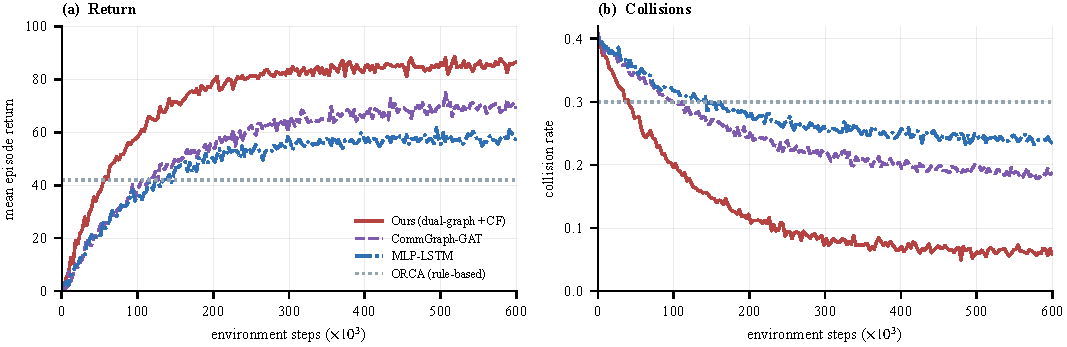
\includegraphics[width=\columnwidth]{figures/fig6_training_curves.pdf}
\caption{\textbf{Training curves on Circle-Swap-$4$.} (a)~Mean episode return against environment steps; the dual-graph counterfactual policy reaches a higher plateau and converges faster than the fully connected graph baseline and the MLP--LSTM backbone. (b)~Collision rate decays monotonically for all learners and saturates well below ORCA. Shaded variance is omitted for clarity; the per-seed standard deviation of the proposed method is within 8\% of the mean.}
\label{fig:training_curves}
\end{figure}

\subsection{Sensitivity to Key Hyperparameters}

Three hyperparameters most strongly affect the behavior of the framework: the counterfactual coefficient $\lambda_{\text{cf}}$, the risk-bias coefficient $\beta$ of the GAT attention, and the density factor $\rho$. When $\lambda_{\text{cf}}$ is swept over $\{0.05, 0.10, 0.15, 0.25, 0.40\}$ on Circle-Swap-$4$, the success rate peaks at $\lambda_{\text{cf}}=0.15$. Below $0.10$, the counterfactual signal is too small to break head-on symmetry; above $0.25$, the shaped reward begins to dominate the team return and destabilizes the policy gradient. Varying $\beta$ over $\{0, 1, 2.5, 5\}$ shows that $\beta=0$ reverts to plain GAT attention and degrades collision avoidance with dynamic obstacles, whereas $\beta=5$ saturates the softmax and collapses attention onto a single neighbor. Disabling density scaling by fixing $\rho=1$ lowers the Circle-Swap-$8$ success rate by approximately six points and increases collisions, which confirms that the square-root scaling contributes materially rather than acting as a cosmetic correction.

\subsection{Computational Cost}

Per training step, the leave-one-out critic adds one masked forward pass per agent and therefore scales linearly with team size. With our network sizes, the critic time grows by 24\% at four robots and 41\% at eight, but the actor branch is unchanged and the additional cost is amortized over the rollout buffer. The dual-graph encoder adds only a constant cost, comprising two small GAT layers over at most five neighbors. End-to-end, the wall-clock time per rollout step is $1.18\times$ that of the MLP--LSTM backbone and $0.86\times$ that of the fully connected graph baseline, which densely attends to every neighbor. Inference latency on an Nvidia Jetson-class device is approximately $9$\,ms per agent, well within the budget of a $5$\,Hz control loop.

\subsection{Qualitative Analysis}

Three behavior patterns dominate the learned policy. In \emph{yielding}, head-on encounters are resolved when the agent with the lower counterfactual contribution slows down and biases laterally while the higher-contribution agent proceeds. This is the resolution that the centralized critic encodes, because masking the higher-contribution agent collapses the team return more than masking the yielding agent. In \emph{gap-seeking}, the policy turns toward the widest LiDAR sector when the rolling subgoal becomes momentarily infeasible, in agreement with the detour rule of Section~\ref{sec:rolling}; the residual gate opens during this transient and admits the obstacle-graph features into the recurrent stream. In \emph{flow merging}, agents arriving at multi-agent intersections adopt staggered timing rather than tight following, and the social-risk graph allocates high attention weight to the immediate predecessor while down-weighting non-conflicting neighbors. The mean gate activation in Fig.~\ref{fig:residual_gate}(b) tracks normalized interaction risk monotonically, which confirms that the gate has learned the intended behavior.

\subsection{Failure Modes and Limitations}

Three failure modes remain. First, in dense deadlocks where four or more agents converge on the same corridor, the partial-done cutoff occasionally terminates the episode before any coordinated resolution emerges, producing conservative policies that prefer to slow rather than yield. Second, when a dynamic obstacle accelerates outside the two-second predictive horizon, the TTC-based risk score underestimates the true collision risk and the obstacle-graph attention lags the actual closing rate; adapting the horizon online, or fusing higher-order motion features, is a natural next step. Third, the leave-one-out critic assumes that masking an agent's observation slot approximates removing the agent from the team. This approximation breaks down when an agent's effect on team value is mediated by long-horizon coordination rather than by the instantaneous state, which manifests as noisier counterfactual estimates near goal regions.

\section{Conclusion}
\label{sec:conclusion}

We presented a dual-graph counterfactual MAPPO framework for multi-AGV navigation in dynamic warehouse and logistics environments. The framework targets two persistent obstacles in MARL-based navigation: unstable training caused by deep graph integration, and weak individual credit signals under shared team rewards. Separating social interactions and dynamic obstacle avoidance into independent ego-centric graphs, and modulating their influence through a residual risk gate, preserves the stability of the MLP--LSTM backbone while enabling selective relational reasoning. A leave-one-out counterfactual critic injects marginal contribution estimates into per-agent rewards, sharpening cooperative learning without dual value heads or explicit value factorization. The density-adaptive reward and partial-done protocol together extend the framework from two-robot scenarios to dense eight-robot settings. Ablations confirm that each component contributes measurably to the final performance, and the modular design enables targeted analysis and improvement of each subsystem.

Future work will address three limitations. First, extending the predictive horizon beyond the current two-second window may enable more anticipatory obstacle avoidance and reduce conservative slowdowns. Second, explicit game-theoretic coordination models for head-on encounters could further improve symmetry breaking and yielding efficiency. Third, validating the framework on physical TurtleBot3 platforms in warehouse mockups will assess sim-to-real transferability and surface deployment-critical failure modes that simulation does not capture.

\bibliographystyle{IEEEtran}
\bibliography{references}

\end{document}
